\documentclass{beamer}

\pdfmapfile{+sansmathaccent.map}


\mode<presentation>
{
	\usetheme{Warsaw} % or try Darmstadt, Madrid, Warsaw, Rochester, CambridgeUS, ...
	\usecolortheme{seahorse} % or try seahorse, beaver, crane, wolverine, ...
	\usefonttheme{serif}  % or try serif, structurebold, ...
	\setbeamertemplate{navigation symbols}{}
	\setbeamertemplate{caption}[numbered]
} 


%%%%%%%%%%%%%%%%%%%%%%%%%%%%
% itemize settings


%%%%%%%%%%%%%%%%%%%%%%%%%%%%
% itemize settings

\definecolor{myhotpink}{RGB}{255, 80, 200}
\definecolor{mywarmpink}{RGB}{255, 60, 160}
\definecolor{mylightpink}{RGB}{255, 80, 200}
\definecolor{mypink}{RGB}{255, 30, 80}
\definecolor{mydarkpink}{RGB}{155, 25, 60}

\definecolor{mypaleblue}{RGB}{240, 240, 255}
\definecolor{mylightblue}{RGB}{120, 150, 255}
\definecolor{myblue}{RGB}{90, 90, 255}
\definecolor{mygblue}{RGB}{70, 110, 240}
\definecolor{mycourseblue}{RGB}{120, 140, 255}
\definecolor{mycourselightblue}{RGB}{245, 250, 255}
\definecolor{mydarkblue}{RGB}{0, 0, 180}
\definecolor{myblackblue}{RGB}{40, 40, 120}

\definecolor{mygreen}{RGB}{0, 200, 0}
\definecolor{mygreen2}{RGB}{245, 255, 230}
\definecolor{mydarkgreen}{RGB}{0, 120, 0}
\definecolor{mydarkgreen}{RGB}{0, 120, 0}


\definecolor{mygray}{gray}{0.8}
\definecolor{mydarkgray}{RGB}{80, 80, 160}
\definecolor{mylightgray}{RGB}{160, 160, 160}

\definecolor{mydarkred}{RGB}{160, 30, 30}
\definecolor{mylightred}{RGB}{255, 150, 150}
\definecolor{myred}{RGB}{200, 110, 110}
\definecolor{myblackred}{RGB}{120, 40, 40}

\definecolor{mypink}{RGB}{255, 30, 80}
\definecolor{myhotpink}{RGB}{255, 80, 200}
\definecolor{mywarmpink}{RGB}{255, 60, 160}
\definecolor{mylightpink}{RGB}{255, 80, 200}
\definecolor{mydarkpink}{RGB}{155, 25, 60}
\definecolor{mywhitepink}{RGB}{255, 240, 240}

\definecolor{mydarkcolor}{RGB}{60, 25, 155}
\definecolor{mylightcolor}{RGB}{130, 180, 250}



\setbeamertemplate{itemize items}[default]

\setbeamertemplate{itemize item}{\color{myblackblue}$\blacksquare$}
\setbeamertemplate{itemize subitem}{\color{mygblue}$\blacktriangleright$}
\setbeamertemplate{itemize subsubitem}{\color{mygray}$\blacksquare$}

\setbeamercolor{palette quaternary}{fg=white,bg=mycourseblue}
\setbeamercolor{titlelike}{parent=palette quaternary}

\setbeamercolor{palette quaternary2}{fg=black,bg=mycourselightblue}
\setbeamercolor{frametitle}{parent=palette quaternary2}

\setbeamerfont{frametitle}{size=\Large,series=\scshape}
\setbeamerfont{framesubtitle}{size=\normalsize,series=\upshape}





%%%%%%%%%%%%%%%%%%%%%%%%%%%%
% block settings

\setbeamercolor{block title}{bg=red!30,fg=black}

\setbeamercolor*{block title example}{bg=mygreen!40!white,fg=black}

\setbeamercolor*{block body example}{fg= black, bg= mygreen2}


%%%%%%%%%%%%%%%%%%%%%%%%%%%%
% URL settings
\hypersetup{
	colorlinks=true,
	linkcolor=blue,
	filecolor=blue,      
	urlcolor=blue,
}

%%%%%%%%%%%%%%%%%%%%%%%%%%

\renewcommand{\familydefault}{\rmdefault}


\newcommand{\mycolor}[1] {
\setbeamercolor{normal text}{fg={#1}} % Recolors standard body text
\setbeamercolor{structure}{fg={#1}}   % Recolors bullets and structure items
\usebeamercolor[fg]{normal text}      % Applies the normal text color immediately
}


\usepackage{amsmath}
\usepackage{mathtools}

\usepackage{cancel}
\usepackage{centernot}

\usepackage{changepage}
\usepackage{subcaption}

\usepackage{qrcode}

\newcommand{\bo}[1] {\mathbf{#1}}
\newcommand{\R}{\mathbb{R}} 
\newcommand{\T}{^\top}     



\newcommand{\mydate}{Fall 2026}

\newcommand{\mygit}{\textcolor{blue}{\href{https://github.com/SergeiSa/Advanced-Control-2026}{github.com/SergeiSa/Advanced-Control-2026}}}

\newcommand{\myqr}{ \textcolor{black}{\qrcode[height=1.5in]{https://github.com/SergeiSa/Advanced-Control-2026}}
}

\newcommand{\myqrframe}{
	\begin{frame}
		\centerline{Lecture slides are available via Github:}
		\bigskip
		\centerline{\mygit}
		\bigskip
		\myqr
	\end{frame}
}


\newcommand{\bref}[2] {\textcolor{blue}{\href{#1}{#2}}}

%%%%%%%%%%%%%%%%%%%%%%%%%%%%
% code settings

\usepackage{listings}
\usepackage{color}
% \definecolor{mygreen}{rgb}{0,0.6,0}
% \definecolor{mygray}{rgb}{0.5,0.5,0.5}
\definecolor{mymauve}{rgb}{0.58,0,0.82}
\lstset{ 
	backgroundcolor=\color{white},   % choose the background color; you must add \usepackage{color} or \usepackage{xcolor}; should come as last argument
	basicstyle=\footnotesize,        % the size of the fonts that are used for the code
	breakatwhitespace=false,         % sets if automatic breaks should only happen at whitespace
	breaklines=true,                 % sets automatic line breaking
	captionpos=b,                    % sets the caption-position to bottom
	commentstyle=\color{mygreen},    % comment style
	deletekeywords={...},            % if you want to delete keywords from the given language
	escapeinside={\%*}{*)},          % if you want to add LaTeX within your code
	extendedchars=true,              % lets you use non-ASCII characters; for 8-bits encodings only, does not work with UTF-8
	firstnumber=0000,                % start line enumeration with line 0000
	frame=single,	                   % adds a frame around the code
	keepspaces=true,                 % keeps spaces in text, useful for keeping indentation of code (possibly needs columns=flexible)
	keywordstyle=\color{blue},       % keyword style
	language=Octave,                 % the language of the code
	morekeywords={*,...},            % if you want to add more keywords to the set
	numbers=left,                    % where to put the line-numbers; possible values are (none, left, right)
	numbersep=5pt,                   % how far the line-numbers are from the code
	numberstyle=\tiny\color{mygray}, % the style that is used for the line-numbers
	rulecolor=\color{black},         % if not set, the frame-color may be changed on line-breaks within not-black text (e.g. comments (green here))
	showspaces=false,                % show spaces everywhere adding particular underscores; it overrides 'showstringspaces'
	showstringspaces=false,          % underline spaces within strings only
	showtabs=false,                  % show tabs within strings adding particular underscores
	stepnumber=2,                    % the step between two line-numbers. If it's 1, each line will be numbered
	stringstyle=\color{mymauve},     % string literal style
	tabsize=2,	                   % sets default tabsize to 2 spaces
	title=\lstname                   % show the filename of files included with \lstinputlisting; also try caption instead of title
}


%%%%%%%%%%%%%%%%%%%%%%%%%%%%
% URL settings
\hypersetup{
	colorlinks=false,
	linkcolor=blue,
	filecolor=blue,      
	urlcolor=blue,
}

%%%%%%%%%%%%%%%%%%%%%%%%%%

%%%%%%%%%%%%%%%%%%%%%%%%%%%%
% tikz settings

\usepackage{tikz}
\tikzset{every picture/.style={line width=0.75pt}}
\usetikzlibrary{shapes.geometric, decorations.markings, positioning, patterns, calc, arrows.meta}


\title{Collocation, Direct Shooting}
\subtitle{Advanced Control}
\author{by Sergei Savin}
\centering
\date{\mydate}



\begin{document}
\maketitle


\begin{frame}{Content}
	\begin{itemize}
		\item Reminder: trajectory optimization problem
		\item Function parametrization: sequence of points and splines
		\item Cubic Hermite splines
		\item Cost function and constraints
		\item Collocation: encoding the dynamics at discrete points
		\item Direct shooting and Runge--Kutta integration
		\item Example: inverted pendulum swing-up
		\item Literature
	\end{itemize}
\end{frame}




\begin{frame}{Reminder: Trajectory Optimization}
	\begin{flushleft}
		Trajectory optimization is the problem of finding a
		\emph{feasible trajectory} that minimizes a chosen
		cost function.
		
		\vspace{0.5em}
		
		For example, we can formulate the problem as
		\[
		\begin{aligned}
			\min_{x(t),u(t),T}\quad
			&
			\Phi\bigl(x(T)\bigr)
			+
			\int_0^T L\bigl(x(t),u(t)\bigr)\,dt
			\\
			\text{s.t.}\quad
			&
			\dot{x}(t)=f\bigl(x(t),u(t)\bigr),
			\\
			&
			x(0)=x_A,
			\qquad
			x(T)=x_B.
		\end{aligned}
		\]
		
		\begin{itemize}
			\item $\Phi(x(T))$ is the \textbf{terminal cost}, which
			penalizes the final state.
			
			\item $L(x(t),u(t))$ is the \textbf{running cost}, which
			penalizes the state and control along the trajectory.
		\end{itemize}
		
		The particular choice of $\Phi$ and $L$ depends on what
		we want the trajectory to achieve.
	\end{flushleft}
\end{frame}


\begin{frame}{Splines}
	\begin{flushleft}
		A \emph{spline} is a smooth piecewise-polynomial function.
		
		\vspace{0.5em}
		
		Given a set of knots
		\[
		t_1 < t_2 < \cdots < t_N,
		\]
		a spline is defined on each interval $[t_i,t_{i+1}]$ as
		\[
		S_i(t)
		=
		a_i
		+b_i(t-t_i)
		+c_i(t-t_i)^2
		+\cdots
		+d_i(t-t_i)^K.
		\]
		
		\vspace{0.5em}
		
		The polynomials are joined smoothly at the knots. For example,
		\[
		S_i(t_i)=S_{i+1}(t_i),
		\]
		\[
		S_i'(t_i)=S_{i+1}'(t_i),
		\qquad
		S_i''(t_i)=S_{i+1}''(t_i),
		\quad \ldots
		\]
		
		Thus, the spline can represent a smooth function
		while using only a finite number of parameters.
	\end{flushleft}
\end{frame}




\begin{frame}{Function parametrization: sequence of points}
	\begin{flushleft}
	
	\begin{figure}
		\centering
		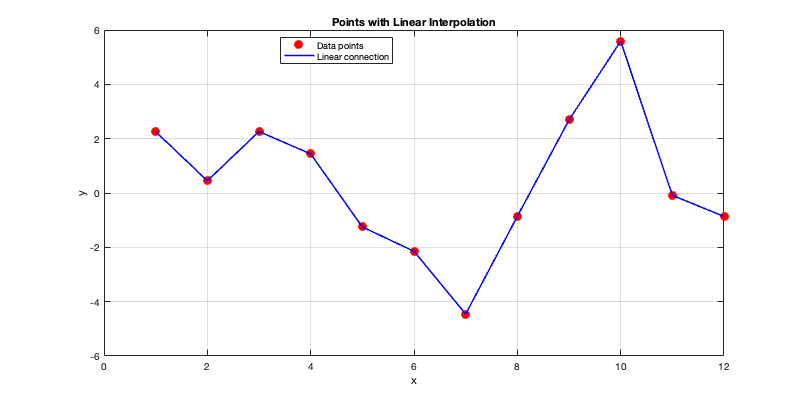
\includegraphics[width=1.1\linewidth]{illustration1}
		\caption{Sequence of points}
		\label{fig:illustration1}
	\end{figure}
	
	\end{flushleft}
\end{frame}




\begin{frame}{Function parametrization: spline}
	\begin{flushleft}
		
		\begin{figure}
			\centering
			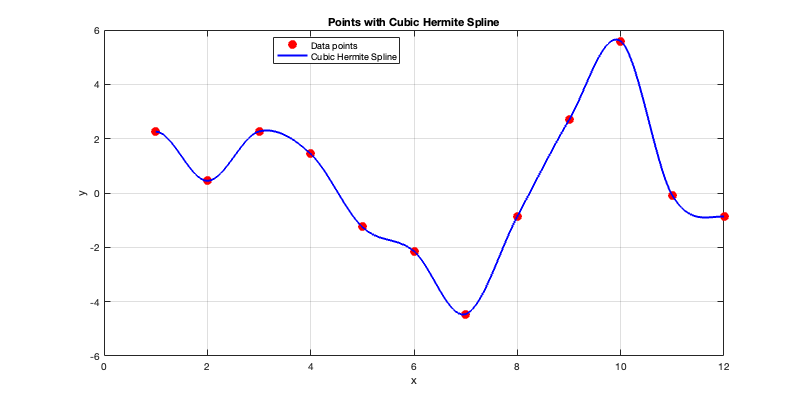
\includegraphics[width=1.1\linewidth]{illustration2}
			\caption{Cubic Hermite Spline}
			\label{fig:illustration1}
		\end{figure}
		
	\end{flushleft}
\end{frame}



\begin{frame}{Cubic Hermite Spline}
	\begin{flushleft}
		A cubic Hermite spline is constructed from third-degree
		polynomials between consecutive knots.
		
		\vspace{0.5em}
		
		For $t\in[t_i,t_{i+1}]$, define the normalized time
		\[
		\tau
		=
		\frac{t-t_i}{t_{i+1}-t_i},
		\qquad
		\tau\in[0,1].
		\]
		
		The spline is
		\[
		S_i(t)
		=
		P_i h_{00}(\tau)
		+
		T_i h_{10}(\tau)
		+
		P_{i+1} h_{01}(\tau)
		+
		T_{i+1} h_{11}(\tau),
		\]
		where $P_i$ is the value and $(t_{i+1}-t_i)T_i$ is the derivative
		at the $i$-th knot. The cubic Hermite basis functions are
\[
\begin{aligned}
	h_{00}(\tau) &= 2\tau^3-3\tau^2+1, & h_{01}(\tau) &= -2\tau^3+3\tau^2, \\
	h_{10}(\tau) &= \tau^3-2\tau^2+\tau, & h_{11}(\tau) &= \tau^3-\tau^2.
\end{aligned}
\]

		
		These basis functions guarantee the prescribed values
		and derivatives at both endpoints.
	\end{flushleft}
\end{frame}



\begin{frame}{Splines in Trajectory Planning}
	\begin{flushleft}
		In trajectory planning, we need to replace continuous
		functions $u(t)$ and $x(t)$ with a finite set of parameters.
		
		\vspace{0.5em}
		
		One option is to represent the functions by their values
		at a finite set of points:
		\[
		u(t)
		\quad\longrightarrow\quad
		\{u_1,u_2,\ldots,u_N\}.
		\]
		
		Alternatively, we can parameterize them using splines:
		\[
		u(t)=u(c,t),
		\]
		where $c$ contains the spline coefficients or knot values.
		
		\vspace{0.3em}
		
		Splines provide a smooth approximation of the trajectory
		and avoid discontinuities.
		
		\vspace{0.3em}
		
		However, smoothness is not always desirable:
		\[
		\text{``hit the gas''}
		\quad\longrightarrow\quad
		\text{``hit the brake''}
		\]
		may naturally require a discontinuous control input.
	\end{flushleft}
\end{frame}


\begin{frame}{Cost Function}
	\begin{flushleft}
		The cost function depends on the problem we are trying
		to solve. However, several common objectives appear
		frequently in trajectory planning.
		
		\vspace{0.5em}
		
		For a problem of moving from $x_A$ to $x_B$ in $N$ steps,
		we may want to:
		
			\textbullet  \, reach the desired final state: $\|x_N-x_B\|^2$;
			
			\textbullet  \, \mbox{keep consecutive states close to each other: $\sum\limits_{i=0}^{N-1}\|x_{i+1}-x_i\|^2$;}
			
			\textbullet  \, use small control inputs: $\sum_{i=0}^{N-1}\|u_i\|^2$.

		
		These objectives can be combined into a single cost:
		\[
		\min
		\quad
		w_1\|x_N-x_B\|^2
		+
		w_2\sum_{i=0}^{N-1}\|x_{i+1}-x_i\|^2
		+
		w_3\sum_{i=0}^{N-1}\|u_i\|^2.
		\]
		
		The weights $w_1,w_2,w_3$ determine the relative
		importance of the different objectives.
	\end{flushleft}
\end{frame}


\begin{frame}{General-Case Quadratic Cost}
	\begin{flushleft}
		A common choice of cost function is a quadratic cost:
		\[
		\min
		\quad
		x_N^\top Q_N x_N
		+
		\sum_{i=0}^{N-1}
		\left(
		x_i^\top Q x_i
		+
		u_i^\top R u_i
		\right),
		\]
		where $Q_N\succeq 0,
		\quad
		Q\succeq 0,
		\quad
		R\succ 0$
		are weight matrices.
		
		\vspace{0.5em}
		
		If $u(t)$ or $x(t)$ is parameterized using a spline,
		we can evaluate the spline at any desired time $t_i$. The evaluation points do not have to coincide with
		the spline knots.
		
		\vspace{0.5em}
		
		For example, if $u(t)=a+bt$,
		then evaluating $J = \sum u_i^2$ at
		\[
		t_i\in\{0,0.5,1\}
		\]
		gives
		\[
		J
		=
		a^2
		+
		(a+0.5b)^2
		+
		(a+b)^2.
		\]
	\end{flushleft}
\end{frame}


\begin{frame}{Constraints}
	\begin{flushleft}
		Trajectory planning problems often include constraints
		that describe what trajectories are physically or
		geometrically feasible.
		
		\vspace{0.5em}
		
		Common examples include:
		\begin{itemize}
			\item Torque limits:
			\[
			|u_i|\leq u_{\max}.
			\]
			
			\item Joint and velocity limits:
			\[
			x_{\min}\leq x_i\leq x_{\max}.
			\]
			
			\item Self-collision constraints.
			
			\item Obstacle and collision avoidance.
			
			\item Contact and grasping constraints.
		\end{itemize}
		
		\vspace{0.5em}
		
		We also commonly impose the initial and final conditions
		as constraints:
		\[
		x_0=x_A,
		\qquad
		x_N=x_B.
		\]
	\end{flushleft}
\end{frame}

\begin{frame}{Collocation}
	\begin{flushleft}
		We are left with the task of encoding the system dynamics:
		\[
		\dot{x}=f(x,u).
		\]
		
		\vspace{0.5em}
		
		\emph{Collocation} enforces the dynamics at a finite
		number of points in time, called \emph{collocation points}.
		
		\vspace{0.5em}
		
		Consider a simple case where $x(t)$ and $u(t)$ are
		represented by their values
		\[
		x_0,x_1,\ldots,x_N,
		\qquad
		u_0,u_1,\ldots,u_{N-1}.
		\]
		
		Approximating the derivative using a finite difference,
		\[
		\dot{x}(t_i)
		\approx
		\frac{x_{i+1}-x_i}{t_{i+1}-t_i},
		\]
		we obtain the collocation constraints
		\[
		\frac{x_{i+1}-x_i}{t_{i+1}-t_i}
		=
		f(x_i,u_i),
		\qquad
		i=0,\ldots,N-1.
		\]
	\end{flushleft}
\end{frame}

\begin{frame}{Collocation: Properties}
	\begin{flushleft}
		The collocation approach to handling the dynamics has
		distinct properties:
		
		\vspace{0.5em}
		
		\begin{itemize}
			\item The dynamics are enforced only at a finite number
			of collocation points.
			
			\vspace{0.5em}
			
			\item The decision variables include the states
			\[
			x_0,x_1,\ldots,x_N
			\]
			and the controls
			\[
			u_0,u_1,\ldots,u_{N-1}.
			\]
			
			\vspace{0.5em}
			
			\item Alternatively, $x(t)$ and $u(t)$ can be represented
			using splines or other parameterizations.
			
			\vspace{0.5em}
			
			\item The resulting optimization problem contains
			explicit constraints representing the system dynamics.
		\end{itemize}
	\end{flushleft}
\end{frame}

\begin{frame}{Direct Shooting}
	\begin{flushleft}
		
		{\small 
		In contrast to collocation, \emph{direct shooting} encodes
		the dynamics through a numerical integration scheme.
		
		\vspace{0.5em}
		
		Given the initial state $x_0$ and the control inputs
		$u_0,u_1,\ldots$, the states are generated by propagating
		the dynamics forward in time.
		
		\vspace{0.5em}
		
		For example, using the forward Euler method,
		\[
		x_{i+1}
		=
		x_i
		+
		f(x_i,u_i)
		(t_{i+1}-t_i).
		\]
		
		Starting from $x_0$, this gives
		\[
		x_1=x_1(u_0),
		\qquad
		x_2=x_2(u_0,u_1),
		\qquad\ldots
		\]
		
		Thus, the states are \emph{expressions of the control
			parameters}, rather than independent decision variables.
		
		\vspace{0.5em}
		
		With Euler integration, this is algebraically equivalent
		to the previous discretized dynamics constraints. The distinction becomes important when more sophisticated
		integration schemes are used.
	}
	\end{flushleft}
\end{frame}


\begin{frame}{Runge--Kutta Integration}
	\begin{flushleft}
		Instead of the Euler method, we can use a higher-order
		integration scheme such as fourth-order Runge--Kutta (RK4).
		
		\vspace{0.5em}
		
		For a time step $h=t_{i+1}-t_i$, define
		\[
		\begin{aligned}
			k_1 &= f(x_i,u_i),\\
			k_2 &= f\left(x_i+\frac{h}{2}k_1,u_i\right),\\
			k_3 &= f\left(x_i+\frac{h}{2}k_2,u_i\right),\\
			k_4 &= f\left(x_i+h k_3,u_i\right).
		\end{aligned}
		\]
		
		\vspace{0.5em}
		
		The state is then propagated according to
		\[
		x_{i+1}
		=
		x_i
		+
		\frac{h}{6}
		\left(
		k_1+2k_2+2k_3+k_4
		\right).
		\]
		
		Thus, in direct shooting, the entire trajectory is
		obtained by repeatedly applying this propagation step.
	\end{flushleft}
\end{frame}
\begin{frame}{Inverted Pendulum: Collocation}
	\begin{flushleft}
		Consider an actuated pendulum with dynamics
		\[
		\dot{\omega}=-\sin(\phi)+u,
		\qquad
		\dot{\phi}=\omega.
		\]
		
		\vspace{0.5em}
		
		We want to move the pendulum from the downward position
		to the upright position: $		\phi_0=0,
		\quad
		\phi_N=\pi,
		\quad
		\omega_0=\omega_N=0.$

		The collocation formulation is
		\[
		\begin{aligned}
			\min_{\phi_i,\omega_i,u_i}\quad
			&
			\sum_{i=0}^{N-1}
			\left[
			w_1(\omega_{i+1}-\omega_i)^2
			+
			w_2(\phi_{i+1}-\phi_i)^2
			+
			w_3u_i^2
			\right]
			\\[0.5em]
			\text{s.t.}\quad
			&
			\frac{\omega_{i+1}-\omega_i}{h}
			=
			-\sin(\phi_i)+u_i,
			\\
			&
			\frac{\phi_{i+1}-\phi_i}{h}
			=
			\omega_i,
			\qquad i=0,\ldots,N-1,
			\\
			&
			\phi_0=0,\quad
			\omega_0=0,\quad
			\phi_N=\pi,\quad
			\omega_N=0,
			\\
			&
			|u_i|\leq u_{\max},
			\qquad i=0,\ldots,N-1.
		\end{aligned}
		\]
		
		Here, $\phi_i$, $\omega_i$, and $u_i$ are all
		optimization variables.
	\end{flushleft}
\end{frame}



\begin{frame}{Inverted Pendulum: Direct Shooting}
	\begin{flushleft}
		We can solve the same trajectory planning problem using
		direct shooting. The decision variables are now only the control inputs: $		u_0,u_1,\ldots,u_{N-1}$. Starting from $		\phi_0=0,
		\quad
		\omega_0=0$, 
		we propagate the dynamics using RK4. The resulting optimization problem is

		\begin{align}
			\min_{u_0,\ldots,u_{N-1}}\quad
			&
			\sum_{i=0}^{N-1}
			\left[
			w_1(\omega_{i+1}-\omega_i)^2
			+
			w_2(\phi_{i+1}-\phi_i)^2
			+
			w_3u_i^2
			\right]
			\\[0.5em]
			\text{s.t.}\quad
			&
			\begin{bmatrix}
				\omega_{i+1}\\
				\phi_{i+1}
			\end{bmatrix}
			=
			\operatorname{RK4}
			\left(
			\begin{bmatrix}
			\omega_i\\
			\phi_i
		\end{bmatrix},
		u_i,h
		\right),
		\\
		&
		\phi_N=\pi,\qquad
		\omega_N=0,
		\\
		&
		|u_i|\leq u_{\max},
		\qquad i=0,\ldots,N-1.
	\end{align}

	
	Here, $\phi_i$ and $\omega_i$ are generated by the
	dynamics and are not independent optimization variables.
\end{flushleft}
\end{frame}



\begin{frame}{Literature}
	
	\begin{itemize}
		
		
		\item Russ Tedrake -- MIT:
		\bref{https://underactuated.mit.edu/trajopt.html}
		{Underactuated Robotics: Trajectory Optimization, ch. 10.}
		
	\end{itemize}
	
\end{frame}



\myqrframe




\end{document}
